\documentclass{article}

% if you need to pass options to natbib, use, e.g.:
%     \PassOptionsToPackage{numbers, compress}{natbib}
% before loading neurips_2020

% ready for submission
% \usepackage{neurips_2020}

% to compile a preprint version, e.g., for submission to arXiv, add add the
% [preprint] option:
%     \usepackage[preprint]{neurips_2020}

% to compile a camera-ready version, add the [final] option, e.g.:
%     \usepackage[final]{neurips_2020}

% to avoid loading the natbib package, add option nonatbib:
\usepackage[sort]{natbib}
\usepackage[final]{neurips_2020}
\usepackage[utf8]{inputenc} % allow utf-8 input
\usepackage[T1]{fontenc}    % use 8-bit T1 fonts
\usepackage{hyperref}       % hyperlinks
\usepackage{url}            % simple URL typesetting
\usepackage{booktabs}       % professional-quality tables
\usepackage{amsfonts}       % blackboard math symbols
\usepackage{nicefrac}       % compact symbols for 1/2, etc.
\usepackage{microtype}      % microtypography
\usepackage{graphicx}       %images

\bibliographystyle{dinat} %abbrvnat
\defcitealias{Kag}{FGVC9}

\title{The Herbarium 2022. Flora of North America}

% The \author macro works with any number of authors. There are two commands
% used to separate the names and addresses of multiple authors: \And and \AND.
%
% Using \And between authors leaves it to LaTeX to determine where to break the
% lines. Using \AND forces a line break at that point. So, if LaTeX puts 3 of 4
% authors names on the first line, and the last on the second line, try using
% \AND instead of \And before the third author name.

\author{%
  Alejandro Barreiro Morante \\
  Department of Computer Science\\
  Technische Universität Wien\\
  \texttt{12134025@student.tuwien.ac.at} \\
  % examples of more authors
  \And
  Patrick Indri 
  \thanks{
  Teacher assigned as supervisor of the project. } \\
  Department of Computer Science\\
  Technische Universität Wien\\
  \texttt{patrick.indri@tuwien.ac.at} \\
}

\begin{document}

\maketitle
 \begin{abstract}
Plants are of fundamental importance to life on Earth. With the threat of climate change advancing, new ideas are needed to combat it. This is where this paper comes in, a solution to the Herbarium 2022 - FGVC9 competition. It consists of identifying plant species through herbarium sheets. This paper details the solution adopted, as well as a study of the machine learning field that comprises it. \end{abstract}

\section{Motivation}\label{motivation}

Nowadays, climate change is already a reality that is being expressed across the globe. The unequivocal increase in average air and ocean temperatures, changes in precipitation patterns, widespread melting of ice and rising sea levels, and other stresses, in particular habitat destruction, have already affected many animal and plant species and could potentially lead to extirpations and possibly extinctions \cite{climchang}. 

According to The World Checklist of Vascular Plants, a comprehensive list of scientifically described plant species, there are approximately 350,000 known vascular plant species and it is estimated that there are still thousands more to be discovered \cite{WCVP}. The last report of the Royal Botanic Gardens on 2020 \cite{kew20}, estimates that 39.4\% of plants are in danger of extinction, a figure already too high in itself but if we also take into account that in its 2016 report, the figure was 20\% \cite{kew16}  the concern is even greater. This speaks out how we need new tools to quicken the pace of species discovery.

In recent years, the need for increased efforts to combat climate change has become even more apparent, and organizations and administrations around the world have adopted various commitments and measures, 
Among this matter, we can handle the climate quandary bit by bit through machine learning contests, which is where the Kaggle competition \citetalias{Kag} addressed in this paper comes into play. 

\section{Introduction}

In botany, Flora is a systematic account of plants of a defined geographical area and provides keys and descriptions of plants for identification. Flora is a tool used to identify plants and can be useful in fields like Biodiversity management or forest, ecosystem, and land management, even for evaluating phytogeography patterns. \cite{flora}

A neural network, or artificial neural network learning algorithm, is a computational learning system that uses a network of functions (neurons), to understand and translate a data input of one form into the desired output. Each neuron has inputs and produces a single output which can be sent to multiple other neurons. The inputs can be the feature values of a sample of external data, such as images or documents, or they can be the outputs of other neurons. The outputs of the final output neurons of the neural net accomplish the task, such as recognizing an object in an image. They have evolved over the years with different architectures and paradigms, which have advanced the state of the art in multiple domains, helping in different ways to solve many real-life problems. 
  
\subsection{The competition}
The Herbarium Challenge competition, sponsored by the New York Botanical Garden, has been running for four consecutive years as a part of a workshop on the image recognition problem, specifically Fine-Grained Visual Categorization, \cite{FGVC}. This problem focuses on differentiating between hard-to-distinguish object classes, the Workshop explores topics related to a lot of different fields, from retrieving the “same products" from a million-scale product database to counting individual animals across temporal sequences of cameras.

This topic focuses on identifying different plant species. The competition is based on a dataset that strives to represent all known vascular plant taxa in North America, only vascular land plants (lycophytes, ferns, gymnosperms, and flowering plants), using images gathered from the flora of 60 different botanical institutions around the world.

It is important to highlight that herbarium sheets result in a significantly affected visual representation of the species, as we can see in Fig.\ref{fig:plants}, dominates a monotonous aspect of brown and dark green content and a modified shape of the leaves, fruits, or flowers due to the drying process and aging. Besides, some of the sheets are surrounded by a black frame and contain handwritten/typewritten texts, institutional stamps, bar codes, and the most recent ones, color bar patterns. Although these elements are very important to taxonomists, they introduce a lot of information that can be misinterpreted by machine learning models. However, we can notice in  Fig.\ref{fig:plants} that the text labels on the specimen images have been blurred to remove category information.

\begin{figure}[h]
    \centering
    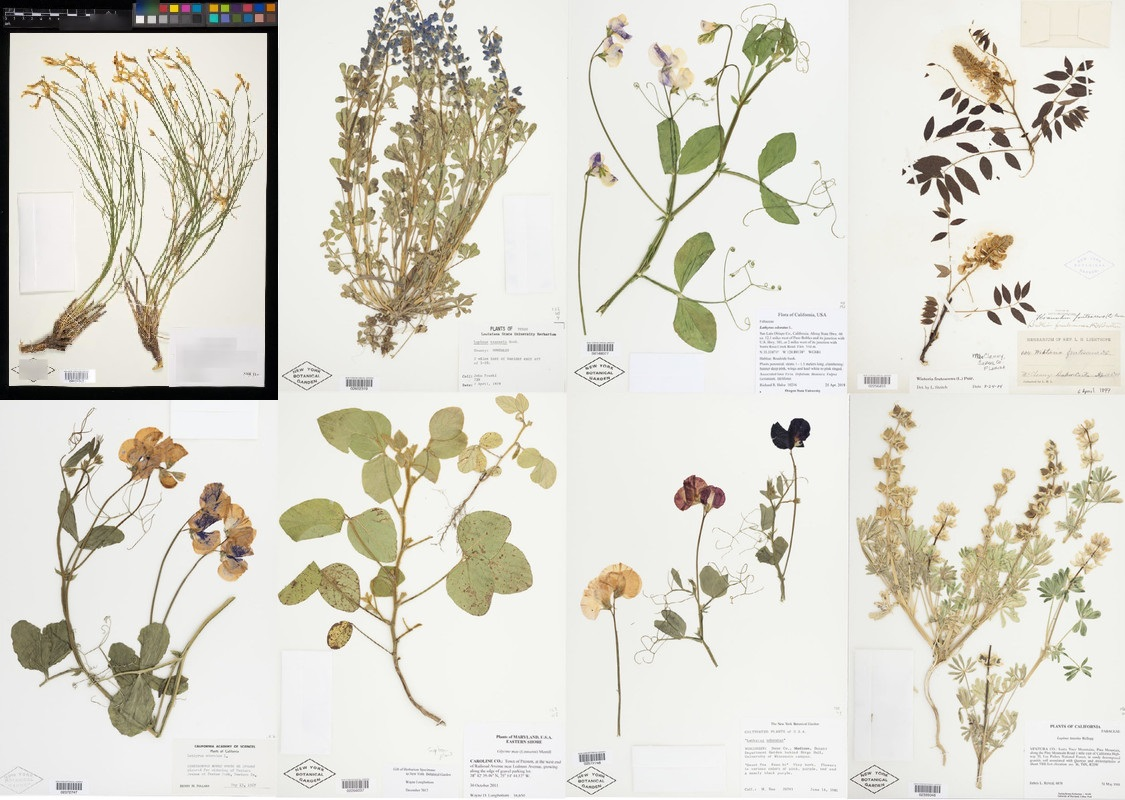
\includegraphics[width=13cm]{plants}
    \caption{Image samples from the dataset}
    \label{fig:plants}
\end{figure}

\subsection{A flora in a Neural Network}

The hypothesis put forward is that the neural network that I will design and train, will encapsulate the flora of North America so our tool can replace the traditional method and be used to determine which names to apply to plant specimens. 

In the following sections, a research on the field will be detailed, followed by the deep learning implementations that have been chosen and developed to approach the objective of the competition, classifying plant taxa according to herbarium sheets.

\section{Related Work}\label{relwork}

Changes in the approaches followed in plant identification and classification have changed by leaps and bounds in recent years. In the first studies on the subject, the approach followed consisted of studying the structure and function of individual organs like leaves and stems \cite{leafvein}. Despite, reporting some interesting results in pattern detection, focusing on the classification of species in such a concrete ecophysiological trait is not sufficient, as the factors shaping phenotype (in biology, visual characteristics that define species and are determined by different factors) are complex. In a nutshell, we could try to analyze completely different taxa (i.e. from different families) that share ecophysiological traits, (i.e. leaves), and the machine learning algorithms would not have any chance to differentiate them, limiting the application of individual organs on species classification \cite{frontiersplants}. 

After the advances in the machine learning for plant classification field which includes the analysis made in the upper paragraph and computational resources, a new paradigm started, identifying plants with all kinds of images that included them began to give promising results. The most popular methods were based on Support Vector Machines \cite{svm} which were based on feature extraction and had really slow progress. 

Nevertheless, years later in the LifeCLEF 2014 plant identification task, the winners presented the usage of a new technology that did not require all the feature extraction progress, simplifying and reducing all the work the computer scientist had to do. They used a convolutional neural network architecture, Alexnet \cite{alexnet}, in a pipeline with an SVM \cite{lifeclef2014}, outperforming by a margin their competitors. After that, the popularization of deep learning was granted, beginning a revolution in the field \cite{story}.

Years later, in 2017, the appearance of a new paper, "attention is all you need" \cite{transformers} introduced a simple but revolutionary concept, the attention mechanism. It can be considered one of the most valuable breakthroughs in Deep Learning research in the last decade, resulting in huge leaps in state-of-the-art performance in different fields, but mainly in Natural Language Processing.

Many works show that transformers matched and even surpassed most CNNs architectures, achieving state-of-the-art performance on most computer vision problems (i.e. Vision Transformer ViT \cite{vit}), demonstrating that they have a larger capacity than the convolutional networks. When a transformer is trained on sufficient data, it has better
performance than CNNs. A possible explanation is that transformers have few prior assumptions about the data structure and that is why they are more flexible than CNNs. However, one counterpart of these low data assumptions is that transformers need more amount of data than CNNs to accomplish their peak of performance, meaning that CNNs perform better on low-scale datasets. Consequently, developing efficient and accessible transformer models for computer vision remains an open problem.\cite{vit1,vit2}

Last but not least, exploring the top scored solutions published over the years on the Herbarium´s competition page, \citetalias{Kag}, can be found interesting approaches adjusted to the problem of classifying taxa based on herbarium images. One of the most common solutions is to ensemble different state of art models, thus building a backbone with them that could bring together the strengths of each to achieve better classifications. \cite{sol1, sol2, sol3}. 

Moreover, a common characteristic of those solutions is the use of the ArcFace loss function \cite{arcface}. The main potential of the function, compared to the cross entropy loss one (a soft-max-based method) is that the last one does not explicitly optimize the feature embedding to enforce higher similarity for intraclass samples (samples that belong to the same class) and diversity for inter-class samples (samples that belong to different classes), which results in lower performance for tasks characterized by intra-class appearance variations, a property that satisfies the species (classes) of our dataset. 

In a more theoretical way, the problem of Softmax is that it does not provide a "safety margin" between the feature vectors of the different classes, it would make two vectors representing two plants of the same species to be as similar as possible while two vectors representing two different classes being as different as possible. The visual representation of Fig.\ref{fig:arcface} provides a helpful representation of the concept.
\defcitealias{embpicture}{[github]}

\begin{figure}[h]
    \centering
    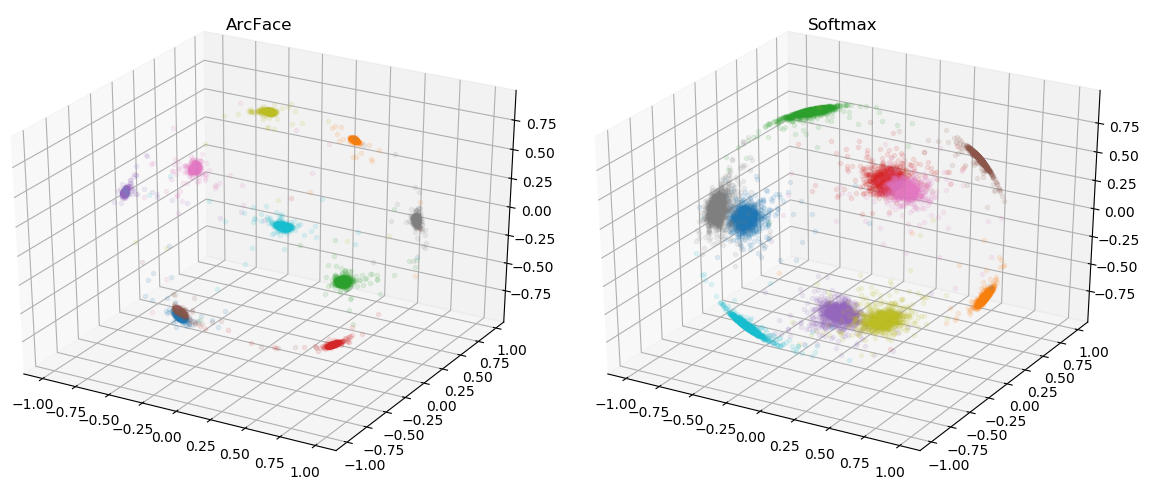
\includegraphics[width=13cm]{arcface}
    \caption{MNIST feature embeddings of the digits using Arcface vs Softmax obtained from \citetalias{embpicture}}
    \label{fig:arcface}

\end{figure}


\section{Methodology}
In order to gain insight into the field, I have been studying some papers on fine-grained image recognition, specifically on plants. This research along with the Pytorch tutorials and the notebooks and discussions published on Kaggle´s competitions have been instrumental in the development of my approach, helping me to educate myself in the field of deep learning as well as discover the state of the art of architectures in the task.

\subsection{Dataset}
Our dataset, “The Herbarium 2022: Flora of North America” comprises 1.050.179 images of 15,501 vascular plants, which constitute more than 90\% of the taxa documented in North America. The number of images per species can be from seven to 100 images. According to the competition, more images are available, but they limited the maximum number in an attempt to ensure sufficient but manageable training data size for the participants.

The dataset includes two JSON files, "train\_metadata" and "test\_metadata", where besides the image´s path, we can find more information about the taxa. The field "categories" in the train metadata contain three levels of hierarchical structure, family - genus - species, with a special condition; we can find multiple categories with the same species name under different genus names because plants are named after the genus-species pair, which are unique. The scientific name is also included, and a new field in this year´s competition; is the phylogenetic distances among genera, under the "distance" attribute.

After the application of a data cleaning process by the organizers, four taxa have been lost, so the "category\_id" are unique but not consecutive (we have 15,501 vascular plants but "category\_id" goes from 0 to 15504). In addition, the number of images per species has been reduced to a maximum of 80 images and a minimum of 5. The  Fig.\ref{fig:long_tail} shows how the dataset follows a long tail distribution, indicating that a large proportion of the species have around 70-80 images while the rest of the species have a low representation of these. This distribution will constitute one of the big challenges of our task; learning to differentiate underrepresented taxa.

\begin{figure}[h]
    \centering
    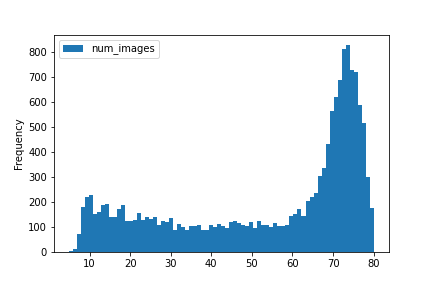
\includegraphics[width=9cm]{long_tail}
    \caption{Histogram showing distribution of training images per taxa.}
    \label{fig:long_tail}

\end{figure}


\subsection{Deep learning}
For solving image-related tasks, the family of machine learning methods that has established itself over recent years is the deep learning architectures,  specifically, convolutional neural networks (CNNs). Predictably, these models have shown improvements in performance on plant species recognition \cite{CNNLifeCLEF} \cite{CNNSDM} \cite{CNNMEE}, compared with previous methods used like Support Vector Machines \cite{svm}. 

The most outstanding feature of these models is their ability to differentiate the visual characteristics of raw pixels in images without being affected by the dimensionality growth of the input data. This special characteristic is reached, thanks to stacking the layers that give the name to the architecture, the convolutional layers. The layers have the effect of filtering the input image with a determined kernel. This transforms the data in such a way that certain features (determined by the shape of the kernel) become more dominant in the output image by having a higher numerical value assigned to the pixels that represent them. These kernels have specific image processing abilities, such as edge detection that highlight the gradient in a particular direction.

\subsection{Transfer learning}
Transfer learning is a strong paradigm that has been introduced in recent years in the field of image recognition tasks. Its goal is to improve the performance of architectures trained with domain-specific training data by transferring knowledge contained in a different but related source domain. This way, we can reduce the amount of training data that most deep learning models need to have a good performance while increasing the performance of the trained models. Its success is based on the fact that the first layers of CNNs deal with the generic features of the images, so we can take advantage of the weights acquired by those layers on similar fields \cite{transferlearning}.

There are two ways to apply transfer learning with deep networks. One possibility is to utilize the pre-trained network as a fixed feature extractor, using the model with the learned weights to obtain features that would be subsequently used in the new problem. Here, the outputs of the network, prior to the last fully-connected layer, constitute features of interest. The other option, and the one we have selected, is to fine-tune the network weights by training the network with the new dataset. \cite{planttransferlearning}

\subsection{Deep learning models}

Here we present the different models that have been selected for approaching the task.

\subsubsection{ResNet}

Following all the improvements that CNNs have brought to image recognition and species classification, we have decided to use one of the most usage extended CNN model, the winner of the ImageNet \cite{Imagenet} classification task on 2015, residual neural network (ResNet) \cite{resnet}. ResNet was chosen because it is a state-of-the-art model, and it is widely used in image classification tasks. Besides, it has been shown that performs decently when counting with limited computation resources (Nvidia GTX 3800).

Residual neural networks are based on the biological fact that neurons can connect with other neurons in layers that are not contiguous, this way, they can skip intermediate layers and increase the number of connections without increasing the computational complexity or the total number of parameters. This feature is translated into controlling the famous known problem of deep neural networks, vanishing gradient. This problem is caused when a network is too deep, the gradients are easily reduced to zero after several applications of the chain rule. The result is that the loss function is affected in a way that the weights of the network are never significantly updated and thus no learning is taking place. The structure of a ResNet-12 is presented on Fig.\ref{fig:resnet}

\begin{figure}[h]
    \centering
    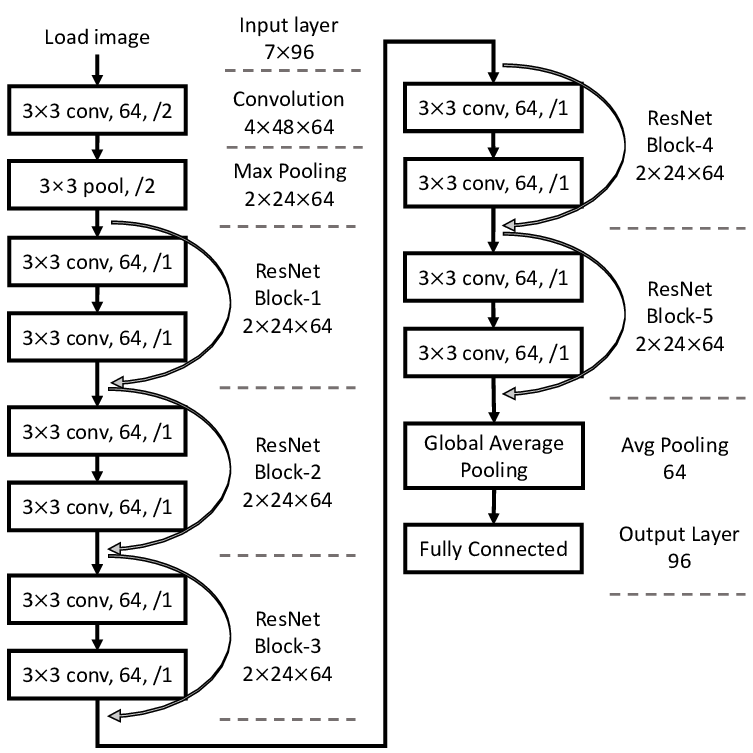
\includegraphics[width=9cm]{resnet12}
    \caption{Image representing the structure of a ResNet that is 12 layers deep, ResNet-12 \cite{resnet12}}
    \label{fig:resnet}

\end{figure}

For approaching the competition, we have selected the pre-trained version of the ResNet architecture with different layer sizes. I must stress that I am working with the pre-trained version that can be found on Pytorch \cite{pyresnet}, having adapted the classification head for the number of herbarium classes, 1505. The model is pre-trained on the dataset ImageNet (ILSVRC) 2012 \cite{Imagenet}, the most used subset of ImageNet. It has 1000  classes and contains 1,281,167 training images, 50,000 validation images and 100,000 test images.

Regarding the fine-tuning of the model, we have selected as the loss function the Cross-Entropy Loss, which is the most extended function for multi-class classification. The reason, in a nutshell, is that when computing the loss, the further away a prediction is from its target, the more the error grows.

The optimizer selected is the stochastic gradient descent, with Momentum and Nesterov Accelerated Gradient. The reason is its wide popularity on Kaggle´s notebooks and discussions of the Herbarium competition, and its stability compared with other optimizers, which is shown on \cite{sgd}. We supported our optimizer with the ReduceLROnPlateau scheduler, which function is to reduce the learning rate of the optimizer after some defined epochs when it has stopped improving.


\subsubsection{Big Transfer BiT}
Delving deeper into the literature, we have found Big Transfer (BiT) \cite{bit}, which attains state-of-the-art performance at multiple tasks on image recognition. The architecture is based on training different ResNets models, with different layer sizes (50, 101, 152), on three different scales of datasets. The first one, BiT-L is trained on the JFT-300M dataset \ to cite{jft}, which contains 300 M noisily labeled images and ~18.000 classes. The second one, BiT-M is trained on the  ImageNet-21k, which contains 14M images with ~21.000 classes, \cite{Imagenet}. The last size model is BiT-S, which is trained on ILSVRC-2012, which contains 1.28M images with 1000 classes \cite{Imagenet}.

Nevertheless, there is a growing discrepancy in image recognition between big-sized models that achieve state-of-the-art performance and models that are affordable in practical applications, therefore, the BiT team has published a compressed model called distilled BiT, thanks to the Teacher-Student architecture, they have managed to replicate a big sized model like BiT-M-R152x2, into small sized ones like ResNet50. The key feature of the Teacher-Student architecture is how it achieves a size reduction without compromising their performance.

\subsection{Image pre-processing}
\label{augmentations}

In this section, we explain the different augmentation techniques we have used to preprocess the images of the dataset. In Fig\ref{fig:plants}, we present some examples before the preprocess.

We have constructed a pipeline with the different configurations that have been found to be successful in research in the field for the augmentation of the images of the dataset. Different experiments have been designed in order to adapt the configurations to the task, taking into account the different types of images available on the dataset.

All the images on a herbarium are digitized with a very high resolution to preserve all the details. Therefore, the organizers resized the images to a maximum of 1000 pixels in the larger dimension. Afterward, we resized the images to a resolution of 380x380 pixels. Subsequently, we have been studying what is the best cropping size, as a lot of images contain a black frame with annotations and a color palette. We have concluded that using a center crop of 350x350 is the ideal cropping as it cleans the noise without erasing taxa information. We have also included a Random Horizontal Flip with a probability of occurring of 50\%. Last but not least, we have calculated the mean and standard deviation of the RGB of all the images of the dataset for applying a normalization, as it has shown to perform better in practice. The visual transformations are presented in Fig.\ref{fig:process}

\begin{figure}[h]
    \centering
    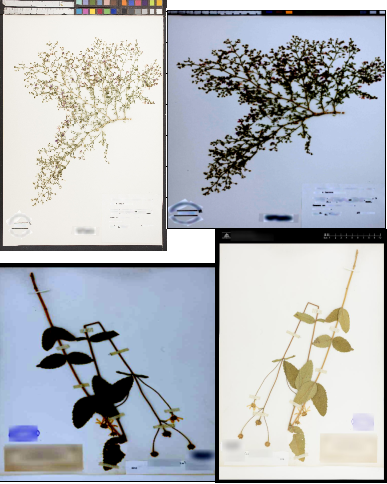
\includegraphics[width=9cm]{process}
    \caption{Image representing the pre and post processed images following the presented pipeline.}
    \label{fig:process}

\end{figure}

On the other hand, it has been suggested the application of Ridge operators to the taxa in order to detect ridge-like structures, such as the plant stems, so the model could learn them better. Nevertheless, we have found struggles, sometimes, it does not provide special information, it induces more noise to the images and it erases all the color of the specimens, being the color an important feature for species classification. Fig. \ref{fig:ridge}

\begin{figure}[h]
    \centering
    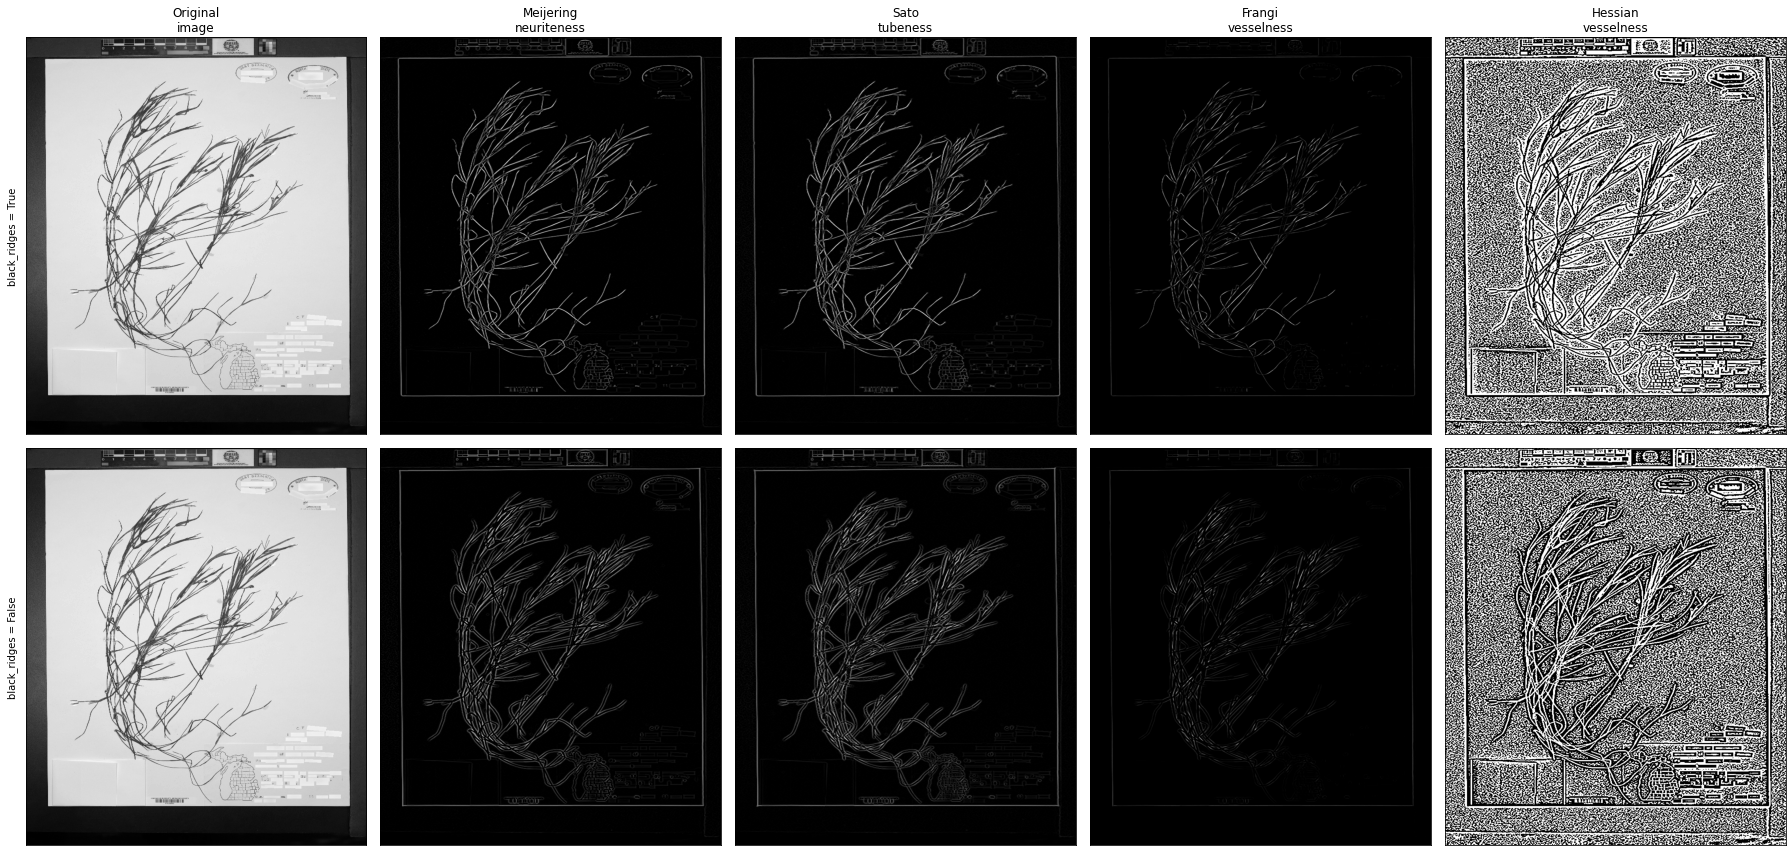
\includegraphics[width=12cm]{ridgeop}
    \caption{Images representing different ridge filters.}
    \label{fig:ridge}
\end{figure}

\subsubsection{Cleaning data}
Analyzing the dataset, I have found different images that do not contain taxa at all, they are just paper boxes with some handwritten text, Fig\ref{fig:badsamples}. We have recognized them as bad samples and we have tried to clean them out from the dataset. The approach taken was to calculate the mean and standard deviation of the RGB and to select the images that had a really low standard deviation. Unfortunately, we found in the process that there are some species that had a very similar std and mean compared with the bad samples, so they were going to be deleted as well, so the idea was discarded.

Other approaches have been tested in order to clean the bad samples, the Luminance distribution analysis, which shows the RGB color distribution could be useful, nevertheless, as we can see in Fig\ref{fig:badsamples}, it is impossible to discard the bad samples because they have a bigger RGB distribution than some examples.

\begin{figure}[h]
    \centering
    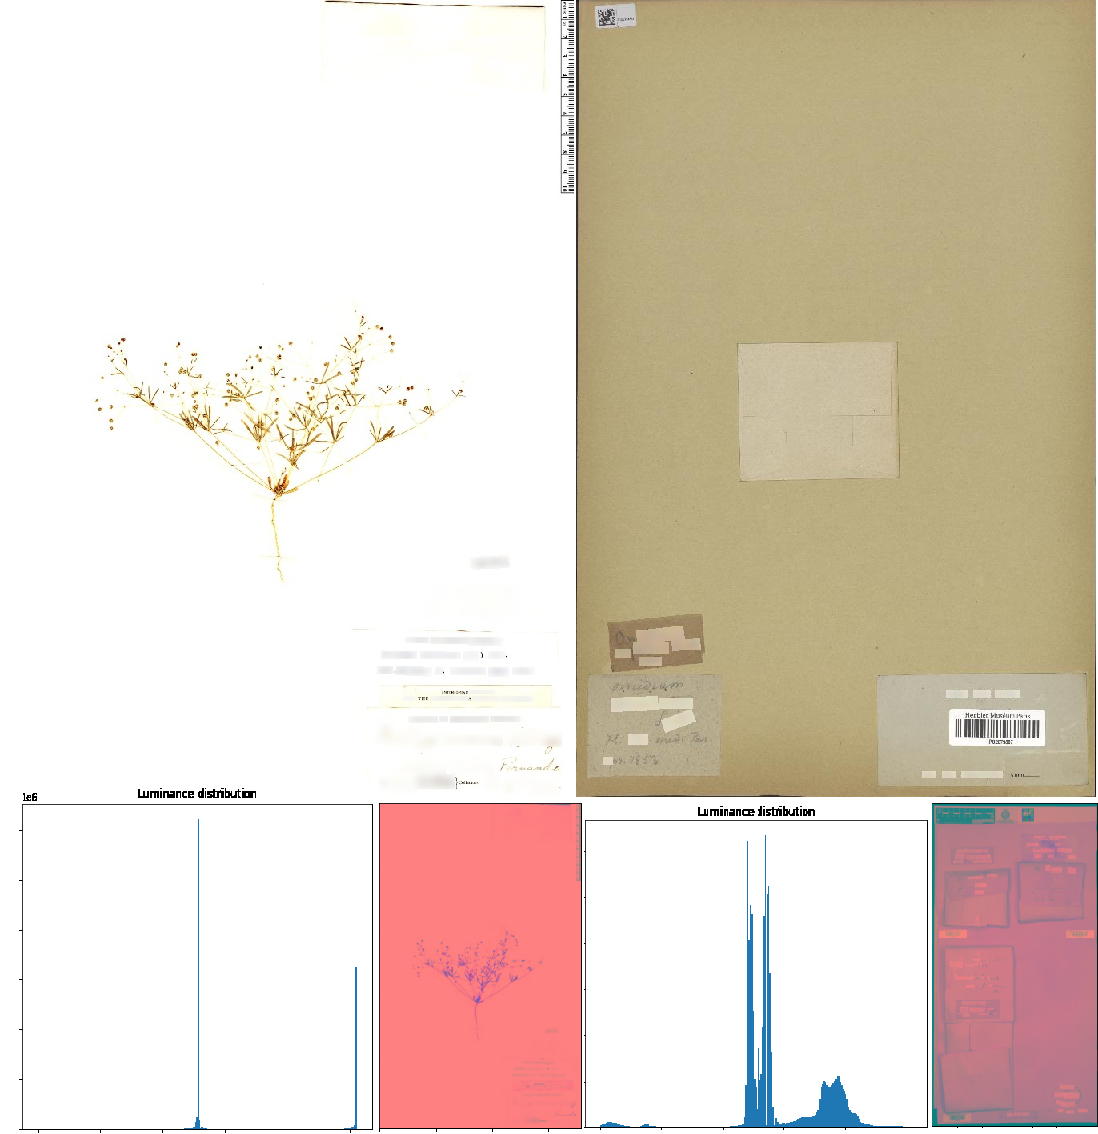
\includegraphics[width=10cm]{badsamples}
    \caption{The image on the left represents a specie with low RGB mean and standard deviation and with respective Luminance histogram and the image on the right represents a bad sample with almost the same mean and std and its respective Luminance histogram.}
    \label{fig:badsamples}

\end{figure}

\subsection{Bottlenecks}
Working in this competition has presented different constraints in order to get results, in this section we will present some of them. The model training has been the biggest bottleneck of the competition, the constraints on the performance of the computer resources have caused the inability to test some architectures like BiT-M and BiT-L, ResNet due to RAM crashes and time constraints. Fixing a low batch size with a mediocre number of epochs has allowed us to get some decent results in the competition.

 \subsubsection{Explainability}
I have tried different explainability techniques for interpreting the model and its results but unfortunately, the computer resources are not enough for computing them. Is important to highlight one downside of Kaggle’s competitions, it does not provide you with the classes of the test set so you can´t focus on the misclassifications of the model without losing training data. 

\section{Results}

All the experiments have been done under the following computer resources: Intel i9 processor, 64 GB RAM, 1 TB SSD, 1 Nvidia RTX 3080, Ubuntu 20.04, seeding all the processes with a seed equal to 9999. 

In order to build the methods with the DataLoaders and the Herbarium data classes, as well as learn the state-of-art of the competition, different notebooks and discussions available on Kaggle's competition page \citetalias{Kag} have been fundamental. \cite{k0,k1,k2,k3}

For the experiments using pre-trained ResNets, the dataset has been split into 2 parts, 80\% for training the architectures and 20\% for validation purposes (n\_splits=5). The splitter that has been used is a Stratified K-Folds cross-validator, which provides train/test indices to split data into train/test sets. It is a variation of k-fold which returns stratified folds: each set contains approximately the same percentage of samples of each target class as the complete set \cite{kfold}.

The ResNet´s pipelines have been built using stochastic gradient descent with a learning rate of 0.5, a momentum of 0.9, and a weight decay of 0.0001 using Nesterov Accelerated Gradient. The scheduler ReduceLROnPlateau has been used with patience of 2, due to the number of epochs (20).

The BiT pipeline uses as augmentation techniques resizing, random cropping, random horizontal flip, and a normalization filter with 510, 480 as resize and crop resolution, and a 0.5 normalizing ratio as mean and std. They use a stochastic gradient descent optimizer, with a Momentum of 0.9, and a learning rate of 0.3. The loss function selected is the Cross-Entropy Loss, and the training is configured to run 20.000 steps as default.

It has been documented comparison between three different models for the fine-grained classification task, reflected in Table \ref{results}. The first two ones have used the same augmentation techniques as defined on \nameref{augmentations}, while the last one has used the augmentation techniques defined in the upper paragraph. The main difference between the augmentation techniques is the resize and cropping ratio, being 512, and 480 respectively for the BiT and 380, and 350 for the ResNets.

\begin{table}[h]
  \caption{Results of the three different experiments}
  \label{results}
  \centering
  \begin{tabular}{llllll}
    \toprule
    Arquitecture     & Private Score    & Public Score  & Batch size  &  Number of epochs    & Time (hours)   \\
    \midrule
    ResNet-18 & 0.61489  &   0.60294  & 64 & 20    & 10 \\
    ResNet-50     & 0.71997 & 0.70747 & 32 & 20  & 22  \\
    BiT-S-101x1     & 0.31922  & 0.31863 & 8  & - & 40 \\
    \bottomrule
  \end{tabular}
\end{table}


With a fixed number of 20 epochs, the model that gave better results was a ResNet50 (50 layers), with a 0.71997 private score and a 0.70747 public score on Kaggle, managing to predict properly more than 2/3 of the species. 

The following graphs represent different logged metrics for the ResNet-50 model. Fig.\ref{fig:acc50} represents the evolution of accuracy, calculated on the validation dataset, over the 20 epochs the model has been trained. Fig.\ref{fig:loss50} shows the loss evolution per the 20 epochs of training, the red line represents the loss evolution over the train set, and the green line the loss evolution over the validation set.  Fig.\ref{fig:losstep} reproduces the train loss evolution per step, reflecting also on the x-axis the
the number of epochs for a better understanding of the steps. It is calculated over the validation set.
\begin{figure}[h]
    \centering
    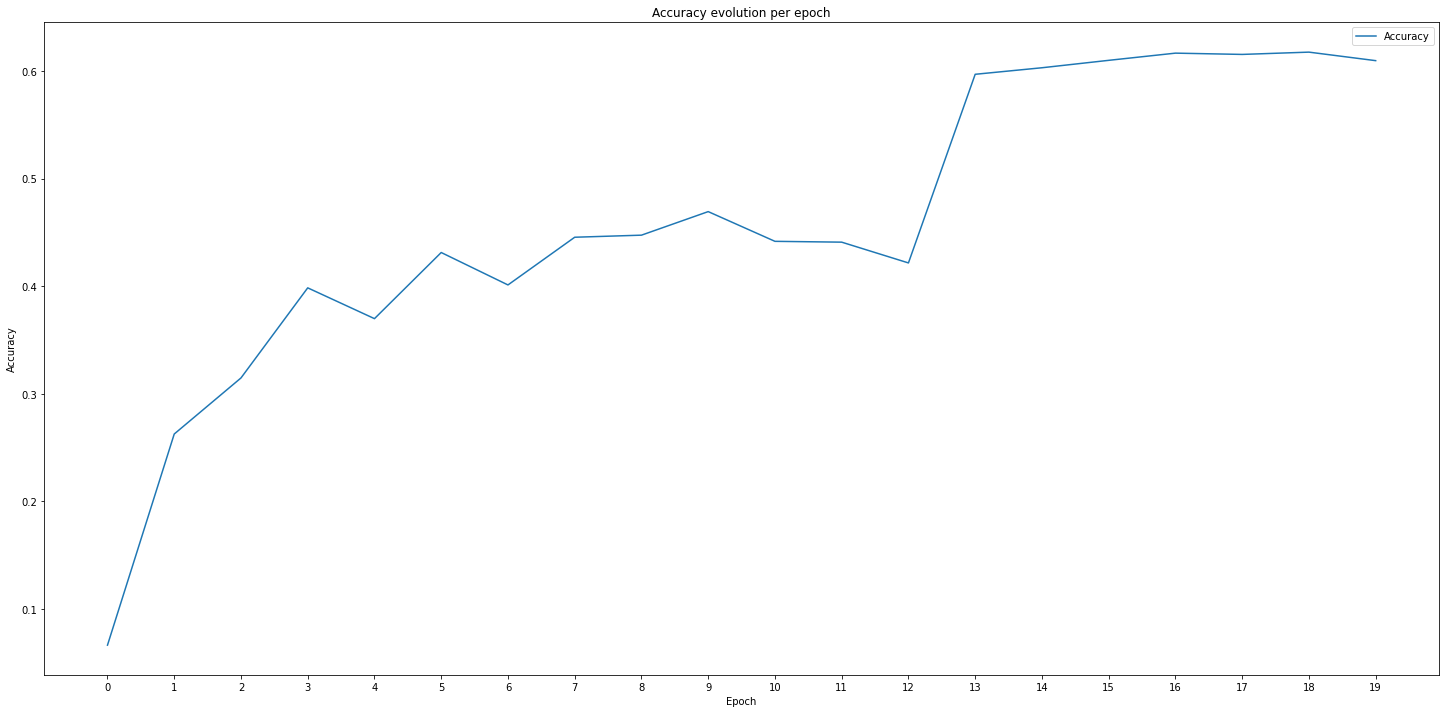
\includegraphics[width=13cm]{acc50}
    \caption{The graph represents the accuracy evolution per epoch}
    \label{fig:acc50}

\end{figure}

\begin{figure}[h]
    \centering
    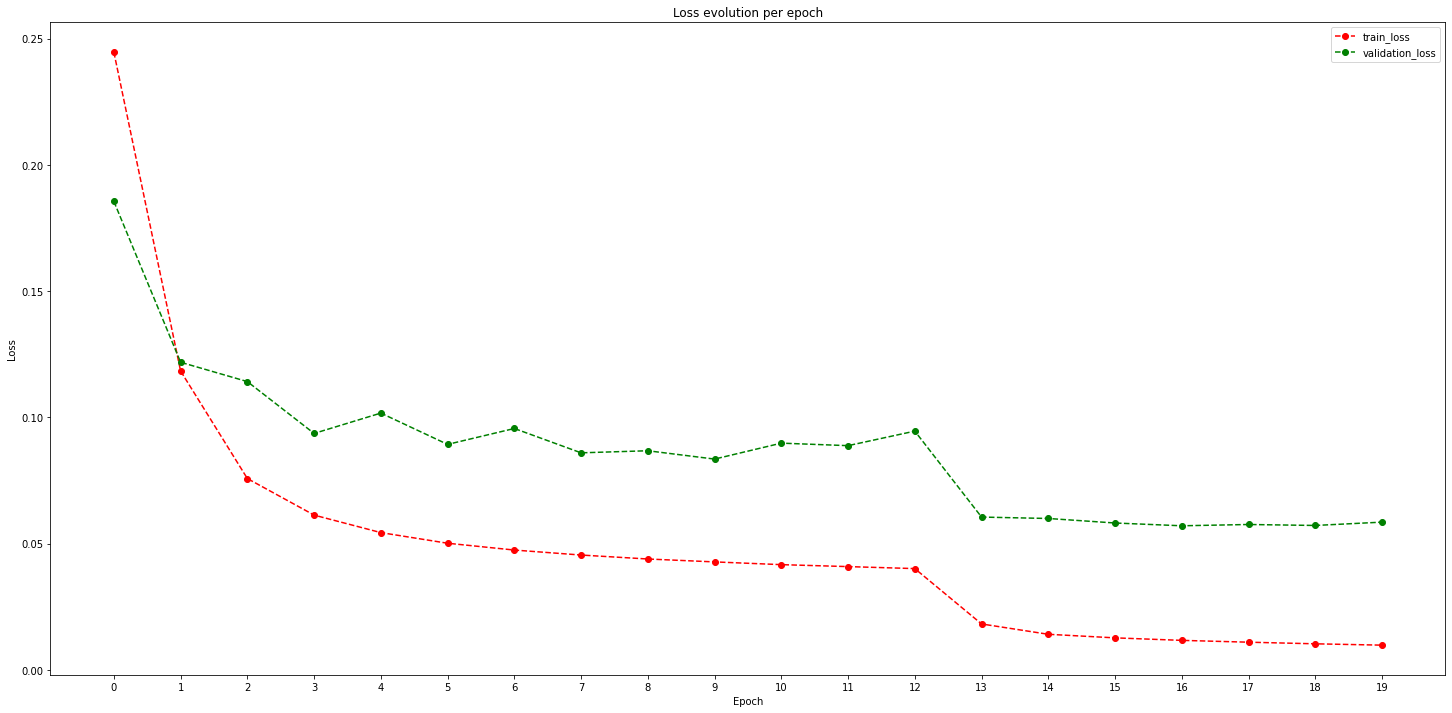
\includegraphics[width=13cm]{loss50}
    \caption{The graph represents the loss evolution per epoch.}
    \label{fig:loss50}

\end{figure}

\begin{figure}[h]
    \centering
    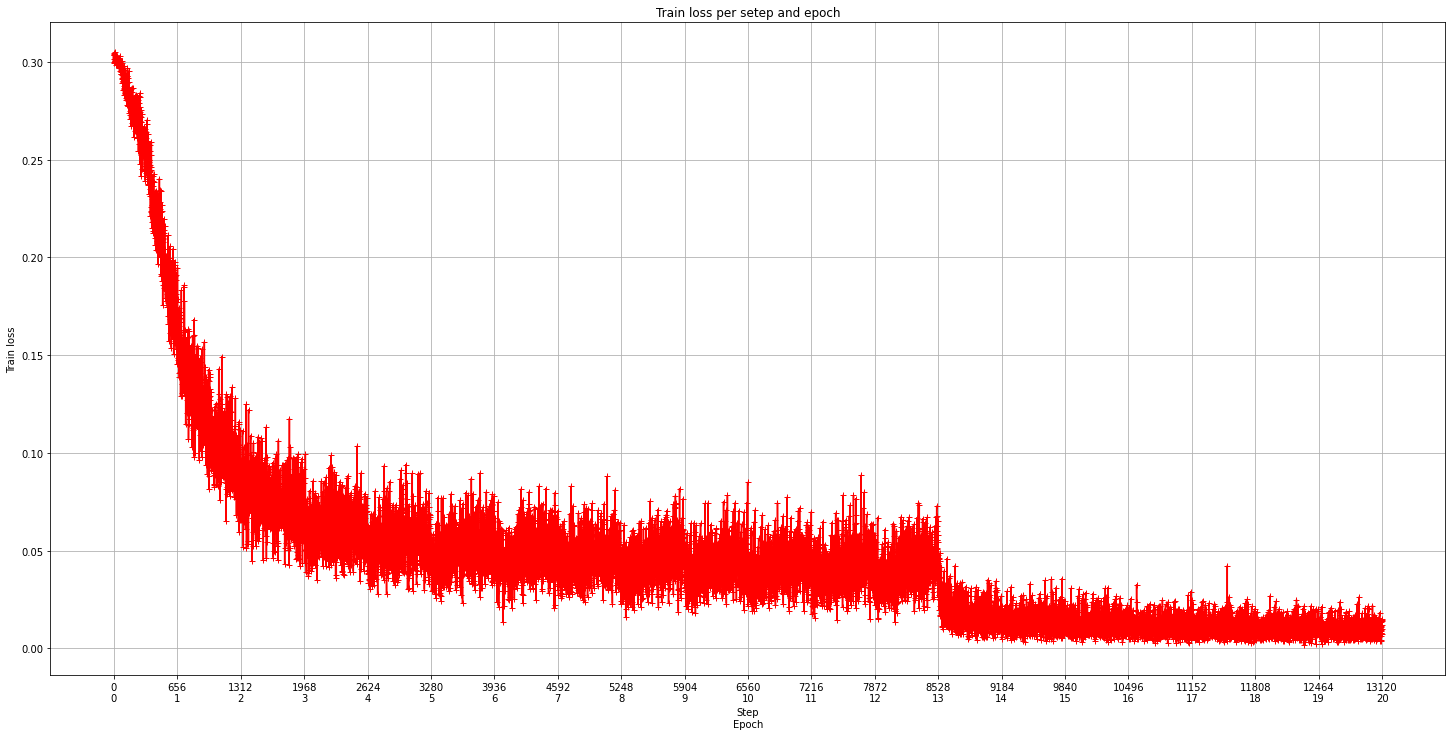
\includegraphics[width=13cm]{losstep}
    \caption{The graph represents the train loss evolution per step, reflecting also on the x axis the number of epoch.}
    \label{fig:losstep}

\end{figure}

\section{Discussion}

In this section we will analyze the different results presented in the last one, pointing out weaknesses and proposing improvements that can be made in order to achieve better results.

The accuracy of ResNet-18 is about 10\% lower than that of its sibling architecture. The explanation for the difference still lies in the number of layers, 18 compared to 50 for its big brother.  In fine-grained classification, in general, as long as sufficient training data is available, the more layers of depth the network has, the better accuracy it will have.

On the other hand, the BiT model has been trained without a validation set, which is probably the reason why the model has such a low score on Kaggle. Due to time restrictions, the model could not be tested, under those circumstances, thus failing to show the true potential of this architecture.

Following the results presented in the graphics, we can stand that the ResNet-50 model has a low improvement margin referring to the number of epochs of training. The accuracy curve \ref{fig:acc50} has flattened out along 6 epochs and neither the loss metric has changed since the 13th epoch \ref{fig:loss50}, meaning that a minimum has been found. Nevertheless, it does not mean that it is impossible to improve the model, a lot of preprocessing augmentation can be done to avoid overfitting.

\section{Conclusion}

This paper has shown that the application of deep learning to the classification of herbarium species is not only possible but really promising. In particular, it shows how the transfer-learning paradigm has a great potential even for fine-grained classification tasks on plants, the images collected on the ImageNet dataset have no relation with the ones of the competition´s dataset, herbarium sheets. 

With the lack of resources that we have disposed of, our model has shown a performance of almost 70\% accuracy, despite having a lot of improvements to be made, all the models can be trained for longer epochs and more augmentation techniques can be tried under those epochs, making robust models that would probably get better accuracy. Talking about the competition, the model would have earned the 36th position if the submissions would have been made on time, a performance higher than the main author of the paper believed he would obtain after the first scores in the competition.

On the other hand, this research helped the main author of the paper to learn and discover the potential of deep learning, a new field for him with enormous dimensions that have found to be surprisingly interesting.

Finally, based on the research carried out, the resources available and the results obtained, it can be affirmed that with a good level of funding and resources, it is possible to obtain a flora in a neural network, and in the close future, discover new taxa and document it with the help of Machine Learning techniques.

\section{Future Work}

This problem is characterized, like most fine-grained recognition problems, by the immense depth with which it can be tackled, coupled with the time constraints that characterize CNNs. Therefore, this section could be extremely extensive, but I will stick to a few key points.  

Training deeper models with a larger number of epochs. There are a few ResNet architectures, like ResNet-101 and ResNet-152 that have not been tested due to time restrictions. These models are promising in a matter of results, due to the nature of the task, a fine-grained problem that needs a lot of detail to differentiate between classes, and the larger the model and the number of epochs, the better the results will be.

Correctly tuning BiT to solve this task. The lack of validation set has affected hugely the BiT performance. 

Analyze the results of the models by creating a test partition from the train images provided. One of the counterparts of all the Kaggle competitions is that they do not provide the test ground truth when the competition is over, making it impossible to contrast what classes are being misclassified by the model.

Search for more optimal explanatory techniques that can explain the models obtained. The resource constraint has made it impossible to apply techniques that have been found in the literature.

As commented on Sec.\ref{relwork}, exploring the first solutions on the Kaggle competition \citetalias{Kag} showed the common usage of backbones with ensemble models, thus incorporating this backbone into the proposed solution will probably increase the performance of the model.
of these years and past ones, one common characteristic is the ensemble of models, building a backbone with different models that bring together the strengths of each to achieve better classifications. On the other hand, trying ArcNet as a loss function instead of CrossEntropyLoss may lead to an improvement of the accuracy as it happened with top-tier solutions in the competition, as commented on Sec.\ref{relwork}

\section{Broader Impact}

Following what has been said on Sec\ref{motivation}, the deployment of a Machine Learning model that could be used to identify taxa could accelerate the pace of species discovery, saving many plant species from extinction. However, the implementation of this tool could affect taxonomists to some extent as it would be doing part of their work. To prevent this from happening, taxonomists should be trained to understand the tool and supervise its operation.

On the contrary, a negative aspect of the Herbarium challenge is the amount of energy and resources consumed by all participants who are likely to be trying similar things. As discussed throughout the paper, deep learning is tremendously demanding in terms of computation and therefore energy, so this challenge contributes to climate change while trying to find tools to mitigate its effects.


\medskip

\small

\bibliography{references}


\end{document}
